\documentclass[11pt]{amsbook}

\usepackage{../HBSuerDemir}	% ------------------------

\begin{document}

% ++++++++++++++++++++++++++++++++++++++
\hPage{b2p1/218}
% ++++++++++++++++++++++++++++++++++++++

\noindent as in (a) there is degeneracy.

\begin{exmp} \
\begin{hEnumerateAlpha}
\item Find the locus of points equidistant from the point $F(0,0,2)$ and the plane $\pi: \quad z=-2$.
\item Sketch the obtained locus
\end{hEnumerateAlpha}
\end{exmp}

\begin{hSolution}
\begin{hEnumerateAlpha}
\item Let $P(x,y,z)$ be equidistant from $F(0,0,2)$ and $\pi: \quad z=-2$. Then

\begin{align*}
    & &&d(P,F) = \sqrt{x^2+y^2+(z-2)^2},\quad d(P,\pi)=\hAbs{z+2}\\
    &\Rightarrow \quad &&x^2+y^2+(z-2)^2 = (z+2)^2\\
    &\Rightarrow \quad &&x^2+y^2 = 8z.\quad \text{(EP)}
\end{align*}

\item Domain:\quad  $\mathbb{R}^2$
\begin{align*}
&\text{Traces}: \quad && \text{xy-trace}: \quad z=0\quad &&&\Rightarrow \quad &&&& x^2+y^2 = 0 \quad &&&&& \text{(origin)}\\
& && \text{xz-trace}: \quad y=0 \quad &&&\Rightarrow \quad &&&& x^2=8z \quad &&&&& \text{(parabola)}\\
& && \text{yz-trace}: \quad x=0 \quad &&&\Rightarrow \quad &&&& y^2=8z \quad &&&&& \text{(parabola)}
\end{align*}

\begin{align*}
&\text{cross sections}: \quad && \text{xy-plane}: \quad z=k\quad &&&\Rightarrow \quad &&&& x^2+y^2 = k \quad &&&&& \text{(circles for k=0)}\\
& && \text{xz-plane}: \quad y=k \quad &&&\Rightarrow \quad &&&& x^2+k^2 =8z \quad &&&&& \text{(parabolas)}\\
& && \text{yz-plane}: \quad x=k \quad &&&\Rightarrow \quad &&&& y^2+k^2=8z \quad &&&&& \text{(parabolas)}
\end{align*}
\end{hEnumerateAlpha}
\end{hSolution}

\begin{figure}[htbp]
        \centering
            \centering
            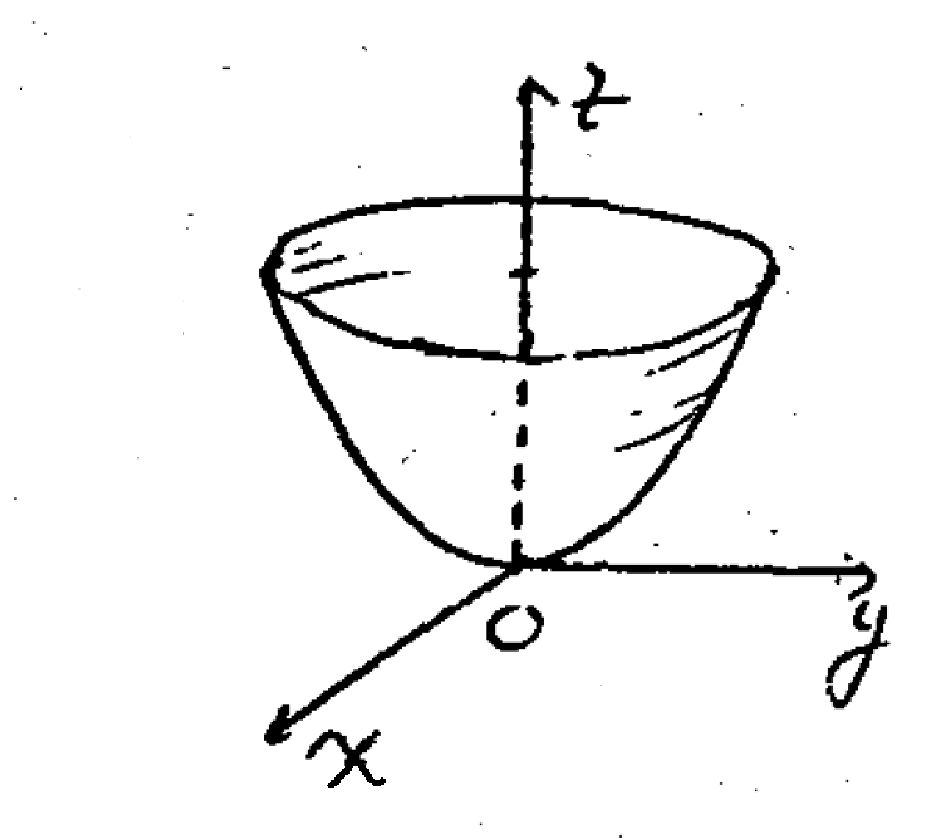
\includegraphics[width=0.2\textwidth]{images/b2p1-218-fig01.pdf}
	        \caption{Locus sketch}
        	\label{fig:LocusSketch}
    \end{figure}   

\subsection{Exercises}

\begin{exercise}
    Plot the following points in a cylindrical coordinate system:
    \[
    A(\frac{\pi}{4}, \enskip3, \enskip4), \quad B(\frac{\pi}{2},\enskip 4,\enskip 1), \quad C(0,\enskip -2, \enskip1), \quad D(0, \enskip0,\enskip 2)
    \]
\end{exercise}
\begin{exercise}
    Plot the following points in a spherical coordinate system:
    \[
    A(\frac{\pi}{4}, \enskip\frac{\pi}{2}, \enskip2), \quad B(\frac{\pi}{2},\enskip \frac{\pi}{4},\enskip 3), \quad C(0,\enskip \frac{\pi}{2}, \enskip-2), \quad D(\frac{\pi}{4}, \enskip\frac{\pi}{4},\enskip 1)
    \]
\end{exercise}
% =======================================================
\end{document}  